%----------------------------------------------------------------------------
\chapter{Rendszerspecifikáció} \label{fejezet3}
%----------------------------------------------------------------------------

\section {Rendszer áttekintése}

A rendszer specifikációit négy nagy részre oszthatjuk fel, amelyek közé tartoznak a felhasználói felület-, a jegyvásárlás-, a felhasználók- és a biztonság specifikációja. Elsőként a felhasználói felület biztosítja a felhasználó és a rendszer közötti kommunikációt. A jegyvásárlás a rendszer központi funkcionalitása, ezáltal a legkomplexebb is. Az alkalmazás lehetővé teszi a több típusú felhasználók hozzáférését a különbőző funkcionalitásokhoz. Végül de nem utolsó sorban a rendszer a bizalmas adatok biztonságát is hivatott kiszolgálni. A specifikációk prezentálására a Visual Paradigm Online felület segítségével hoztam létre a szükséges diagramokat.

\section {Felhasználói felület}

A rendszer felhasználói felülete egy webes alkalmazás felülete, amelyet a frontend technológiák segítségével valósítottam meg. A felületnek az a célja, hogy egyszerű és intuitív legyen, így a felhasználók könnyen tudnak navigálni rajta és megtalálják a kívánt jegyeket.

\subsection {Felhasználói követelmények}

A weboldal használatára háromféle felhasználótípust hoztam létre, amelyek különböző jogosultságokkal rendelkeznek:
\begin{itemize}
	\item Első kategória (\ref{abra:useCaseNA})
	\item Második kategória (\ref{abra:useCaseA})
	\item Harmadik kategória ()
\end{itemize}



\begin{figure}[!h]
	\centering
	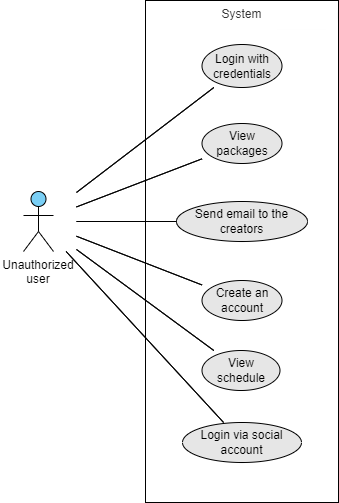
\includegraphics[scale=0.7]{images/useCaseNA}
	\caption{Use case diagram - Nem bejelentkezett felhasználó}
	\label{abra:useCaseNA}
\end{figure}

\begin{figure}[!h]
	\centering
	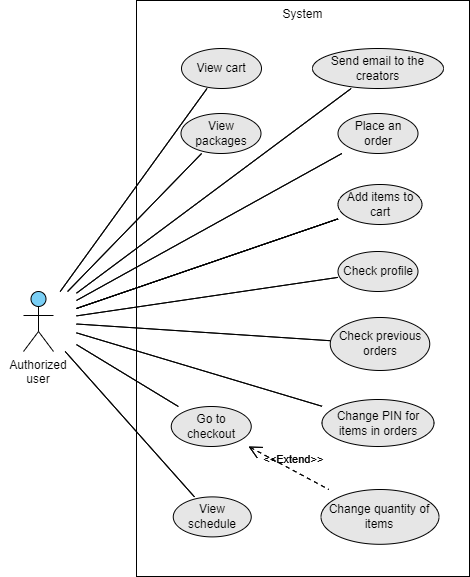
\includegraphics[scale=0.7]{images/useCaseA}
	\caption{Use case diagram - Bejelentkezett felhasználó}
	\label{abra:useCaseA}
\end{figure}
\pagebreak

	\begin{align}
	x&=1+1+1+1\\
	&=4.
\end{align}

	\begin{align}
	y&=mx+b\nonumber\\
	z&=nw+c.
\end{align}

			\begin{align}
	\int_0^1\sum_a^b\prod_\alpha^\beta.
\end{align}
	\begin{align*}
	\frac{12}{34}.
\end{align*}
\subsection {Matlab - \href{https://www.mathworks.com/help/matlab/ref/ode45.html}{ode45}} \label{MatlabOde45}

A Matlab egy programcsomag és egyben egy technikai nyelv is, mely magas szinten lehetőséget biztosít számítások elvégzésére, modellezésre, szimulációra, megjelenítésre, vizualizációra és számos más hasznos mérnöki munka elvégzésére. Esetünkben a legfontosabb, hogy könnyedén tudunk közönséges differenciálegyenleteket megoldani az ode45 program segítségével. Emellett az eredményeket egy jól megtervezett felületen ki is tudjuk ábrázolni. Az alábbi példában jól látható, hogy milyen egyszerű és kényelmes a használata:

\begin{lstlisting}[caption={Matlab példakód diff. egyenlet megoldására.}, captionpos=b]
	f = @(t,y) y;
	t = [0 10];
	y0 = 1.0;
	ode45(f, t, y0);
	plot(t, y(:));
\end{lstlisting}


A fenti bemenetre $ n = 100 $ - szor lefuttattuk az algoritmust és a következő időeredményeket kaptuk:
\begin{itemize}
	\item Futási idők \textbf{átlaga}: $ 0.0043 $ sec
	\item Futási idők \textbf{minimuma}: $ 0.0026 $ sec
	\item Futási idők \textbf{maximuma}: $ 0.1504 $ sec
\end{itemize}




\begin{center}
\smartdiagram[flow diagram:horizontal]{Edit,
	\LaTeX, Bib\TeX/ biber, make\-index, \LaTeX}
\end{center}

\subsection {Boost - \href{http://headmyshoulder.github.io/odeint-v2/}{Odeint}} \label{BoostOdeint}

Egy másik előre megírt közönséges differenciálegyenlet megoldó a Boost könyvtárcsomag Odeint nevezetű könyvtára. Ez egy modern C++ nyelven írt csomag, lényeges jellemzői, hogy \textbf{nagy teljesítményre} képes és \textbf{nagyon magas szinten} (absztraktan - Template Metaprogramming) van megírva, így \textbf{rugalmas} és könnyen integrálható különböző rendszerekbe. Emellett rugalmas a bementi adatok típusát illetően is. Ugyanakkor jó tudni, hogy ez a nagyon absztrakt megvalósítás hátrány is lehet, mert bizonyos esetekben nagyon nehéz megérteni vagy megoldani egy felmerülő problémát. Most lássunk egy egyszerű példát a használatára:

\begin{lstlisting}[caption={Odeint példakód.}, captionpos=b, language = C++]
#include <iostream>
#include <boost/numeric/odeint.hpp>

using namespace std;
using namespace boost::numeric::odeint;

typedef runge_kutta_dopri5<double> stepper_type;

void rhs( const double x , double &dxdt , const double t ) {
	dxdt = 3.0/(2.0*t*t) + x/(2.0*t);
}

void write_cout( const double &x , const double t ) {
	cout << t << '\t' << x << endl;
}

int main() {
	double x = 0.0;    
	integrate_adaptive( make_controlled( 1E-12 , 1E-12 , stepper_type() ) ,
	rhs , x , 1.0 , 10.0 , 0.1 , write_cout );
}
\end{lstlisting}
\pagebreak
Az előző kódrészlet eredménye a következő:



\begin{itemize}
	\item Futási idők \textbf{átlaga}: $ 0.0989 $ sec
	\item Futási idők \textbf{minimuma}: $ 0.09 $ sec
	\item Futási idők \textbf{maximuma}: $ 0.099 $ sec
\end{itemize}

\section {Általam megvalósított szoftverek} \label{fejezet3_2}

\begin{lstlisting}[caption={Matlab kód ode45 használata nélkül.}, captionpos=b, language = Matlab]
function [yy, tt, timeSpent] = fun_dopri45(f, y0, t0, tf, tolerance)
	...
	while t < tf
		if (t+h >= tf)
			h = tf-t;
		end
		
		% Calculate k1, k2, ... , k7
		k1 = h*feval(f, t+h*C(1), y);
		k2 = h*feval(f, t+h*C(2), y + A2(1)*k1);
		...
		k7 = h*feval(f, t+h*C(7), y + A7(1)*k1 + A7(3)*k3 + ... + A7(6)*k6);
		
		% Calcaulate the next point
		yt = y + A7(1)*k1 + A7(3)*k3 + A7(4)*k4 + A7(5)*k5 + A7(6)*k6;
		% Calculate the error
		err = abs(E(1)*k1 + E(3)*k3 + ... + E(7)*k7);
		
		if max(err) < tolerance
			t = t + h;
			y = yt;
			...
		end
		
		% Calculate optimal step size
		scale = 1.25*(maxErr/tolerance)^(1/5);
		if scale > 0.2
			h = h / scale;
		else
			h = 5.0*h;
		end
	end
end
\end{lstlisting}

\begin{itemize}
	\item Futási idők \textbf{átlaga}: $ 0.0043 $ sec
	\item Futási idők \textbf{minimuma}: $ 0.0058 $ sec
	\item Futási idők \textbf{maximuma}: $ 0.0287 $ sec
\end{itemize}

A következő szoftvert, amit bemutatok \textbf{Java} nyelven írtam objektum orientáltan, a fejlesztés során pedig Eclipse fejlesztői környezetet használtam. Ez a szoftver három egységből áll: fő -, differenciálegyenlet megoldó - és kifejezés kiértékelő egység (ezt a legnehezebb megvalósítani vagy megtalálni a megfelelő könyvtárat). Az alkalmazás nem rendelkezik grafikus felhasználói felülettel, a bemeneti adatokat egy szöveges állományból olvassa be (amelynek jól meghatározott szerkezete van) és a kívánt eredményeket a standard kimenetre írja ki. A kifejezés kiértékelő egység megírásánál felhasználtam egy előre elkészített Java könyvtárat, melyet \href{http://www.singularsys.com/jep/}{\textit{JEP}}-nek neveznek. A szoftverben arra használtam fel, hogy egy sztringként megadott kifejezést kiértékeltem és elvégeztem a segítségével. Mindezt úgy csinálja, hogy a háttérben felépít egy kifejezésfát, aminek a leveleiben lesznek az értékek, csúcsaiban a műveletek, zárójelek, stb. (lásd az alábbi ábrát):



\begin{itemize}
	\item Futási idők \textbf{átlaga}: $ 0.1422 $ sec
	\item Futási idők \textbf{minimuma}: $ 0.123 $ sec
	\item Futási idők \textbf{maximuma}: $ 0.341 $ sec
\end{itemize}

Harmadiként lássuk a \textbf{C++ szoftvert}, amelyet szintén objektum orientáltam valósítottam meg. Ennek a szoftvernek a szerkezete hasonló a Java szoftver szerkezetéhez. Ebben az esetben is szükség volt egy kifejezés kiértékelő könyvtárra, hogy ne kelljen egy sajátot írni. Először kipróbáltam egy \href{http://beltoforion.de/article.php?a=muparser}{\textit{muparser}} nevű könytárat, aztán egy másikat is, aminek \href{https://exprtk.codeplex.com/}{\textit{ExprTk}} (Expression Toolkit Library) a neve. Fontos elmondani, hogy mindkét könyvtár ingyenesen elérhető és használható. Az első könyvtárat nehezebb volt hozzáadni a szoftverhez és mivel több fájlból állt több időbe került a fordítása is. A legfőbb ok, amiért mégis a másodikat használtam az volt, hogy jelentősen gyorsabb és hatékonyabb volt az én szoftveremben. Tehát végül az \textit{ExprTk} könyvtárat használtam a jobb teljesítménye és könnyebb integrálhatósága miatt.


\begin{itemize}
	\item Futási idők \textbf{átlaga}: $ 0.1086 $ sec
	\item Futási idők \textbf{minimuma}: $ 0.096 $ sec
	\item Futási idők \textbf{maximuma}: $ 0.214 $ sec
\end{itemize}

Végül nézzük meg az utolsó, Dormand-Prince módszeren alapuló szoftvert, amely egy \textbf{Android alkalmazás}. Mint tudjuk napjainkban a mobileszközök nagyon elterjedtek és teljesítményük is jelentősen megnőtt, lassan felveszik a versenyt a személyi számítógépekkel. Ezért mindenképp szerettem volna az algoritmust megvalósítani mobileszközökre is és megnézni itt is a teljesítményt. Mivel az Android alkalmazások fejlesztésénél Java nyelvet használunk, így könnyű dolgom volt, hiszen a Java szoftverből át tudtam venni a már jól megírt és elkülönített osztályokat. Ugyanazt a \textit{JEP} könyvtárat használtam itt is a kifejezések kiértékelésére, így majd az eredmények összehasonlítását is könnyebbé tettem. A Java és C++ szoftverrel ellentétben rendelkezik egy kis grafikus felhasználói felülettel, de a bemeneti adatokat itt is egy szöveges állományból olvassuk be, mert nem túl kényelmes azt a sok számadatot, meg egyenletet beviteli mezőkön keresztűl beírni.


\begin{itemize}
	\item Futási idők \textbf{átlaga}: $ 37.9015 $ sec
	\item Futási idők \textbf{minimuma}: $ 31.116 $ sec
	\item Futási idők \textbf{maximuma}: $ 70.876 $ sec
\end{itemize}

\section {Szoftverek összehasonlítása} \label{fejezet3_3}

Az előző alfejezetekben ismertettem a már létező Dormand-Prince módszeren alapú differenciálegyenlet megoldók közül kettőt és négy saját megvalósítást is. Mindegyik esetében láthattunk futási időket és számadatokat, azonban nem láttuk ezeket egymás mellett. Ebben az alfejezetben összegezzük és összehasonlítjuk a kapott eredményeket.

Fontos, hogy minden algoritmust ugyanazon a hardveren teszteljünk, mert csak így reálisak és összehasonlíthatóak a mérési adatok. Esetünkben használt hardver konfigurációja:
\begin{itemize}
	\item Intel Core i5-7200U, 2.50 GHz processzor, 8.00 GB RAM memória
\end{itemize}
Természetesen az Android alkamazást csak mobileszközökön lehetett vizsgálni, itt két készüléket használtam a tesztelésre:
\begin{itemize}
	\item Motorola Moto E2, Quad-core 1.2 GHz processzor, 1 GB RAM memória
	\item Samsung Galaxy Core Prime, Quad-core 1.2 GHz processzor, 1 GB RAM memória
\end{itemize}


\begin{table}[h!]
	\centering
	\begin{tabular}{ | l | c | c | c | c |}
		\hline 
		\textbf{Technológia} & \textbf{Átlagidő (s)} & \textbf{Min. idő (s)} & \textbf{Max. idő (s)} & \textbf{Hardver}\\
		\hline
		Matlab - ode45 & $ 0.0032 $ & $ 0.0029 $ & $ 0.0038 $ & Intel Core i5\\
		\hline
		Boost - Odeint & $ 0.0989 $ & $ 0.0900 $ & $ 0.1290 $ & Intel Core i5\\
		\hline
		Matlab & $ 0.0062 $ & $ 0.0060 $ & $ 0.0066 $ & Intel Core i5\\
		\hline
		Java & $ 0.2224 $ & $ 0.1970 $ & $ 0.3020 $ & Intel Core i5\\ 
		\hline
		C++ & $ 0.1047 $ & $ 0.1010 $ & $ 0.1240 $ & Intel Core i5\\
		\hline
		Android & $ 37.9015 $ & $ 31.1160 $ & $ 70.8760 $ & Moto E2\\
		\hline
		Android & $ 35.9987 $ & $ 29.4200 $ & $ 87.6120 $ & Core Prime\\
		\hline
	\end{tabular}
	\caption{Mérési eredmények  $ n = 10 $ tesztesetre.}
	\label{tablazat1}
\end{table}

\begin{table}[h!]
	\centering
	\begin{tabular}{ | l | c | c | c | c |}
		\hline 
		\textbf{Technológia} & \textbf{Átlagidő (s)} & \textbf{Min. idő (s)} & \textbf{Max. idő (s)} & \textbf{Hardver}\\
		\hline
		Matlab - ode45 & $ 0.0043 $ & $ 0.0026 $ & $ 0.1504 $ & Intel Core i5\\
		\hline
		Boost - Odeint & $ 0.0912 $ & $ 0.0900 $ & $ 0.0990 $ & Intel Core i5\\
		\hline
		Matlab & $ 0.0067 $ & $ 0.0058 $ & $ 0.0287 $ & Intel Core i5\\
		\hline
		Java & $ 0.1422 $ & $ 0.1230 $ & $ 0.3410 $ & Intel Core i5\\ 
		\hline
		C++ & $ 0.1086 $ & $ 0.0960 $ & $ 0.2140 $ & Intel Core i5\\
		\hline
		Android & $ - $ & $ - $ & $ - $ & Moto E2\\
		\hline
		Android & $ - $ & $ - $ & $ - $ & Core Prime\\
		\hline
	\end{tabular}
	\caption{Mérési eredmények  $ n = 100 $ tesztesetre.}
\end{table}



\section {Differenciálegyenletek megoldása GPU-n} \label{fejezet3_4}


A továbbiakban nézzük meg a két algoritmus magjának szekvenciális és párhuzamosított változatait:
\begin{lstlisting}[caption={Euler módszer szekvenciális kód.}, captionpos=b, language = C++]
for (int i = 0; i < numberOfVariables; ++i) {
	mResult.at(i)[j + 1] = mResult.at(i)[j] + mInputs->getStepSize() *
	(mFunctionsParsers.at(i)->computeFunctionValue(values));
}
\end{lstlisting}

\begin{lstlisting}[caption={Euler módszer párhuzamosított kód.}, captionpos=b, language = C++]
__global__ void computeFunctionsValuesKernel(double* resultValues,
double* previousValues, double* functionValues, double stepSize, int N) {
	int i = threadIdx.x;
	
	if (i < N) {
		resultValues[i] = previousValues[i] + stepSize * functionValues[i];
	}
}
\end{lstlisting}

\begin{lstlisting}[caption={Runge-Kutta módszer szekvenciális kód.}, captionpos=b, language = C++]
for (int k = 0; k < numberOfVariables; ++k) {
	mResult.at(k)[i + 1] = mResult.at(k)[i] + (mInputs->getStepSize() / 6)*
	(K[0][k] + 2 * K[1][k] + 2 * K[2][k] + K[3][k]);
}
\end{lstlisting}

\begin{lstlisting}[caption={Runge-Kutta módszer párhuzamosított kód.}, captionpos=b, language = C++]
__global__ void computeValuesKernel(double* resultValues, double* K,
double* previousValues, double stepSize, int numberOfVariables) {
	int i = threadIdx.x;
	
	if (i < numberOfVariables) {
		resultValues[i] = previousValues[i] + ((stepSize / 6) *
		(K[i] + 2 * K[i + 1 * numberOfVariables] +
		2 * K[i + 2 * numberOfVariables] + K[i + 3 * numberOfVariables]));
	}
}
\end{lstlisting}

Nézzünk meg pár mérési eredményt a következő differenciálegyenlet rendszerre:
\begin{align}
	\begin{cases}
		y_{1}'(t, y) = y_{1} \\
		\vdots \\
		y_{n}'(t, y) = y_{n}\\
		y_{1}'(t_{0}) = 1.0 \\
		\vdots \\
		y_{n}'(t_{0}) = 1.0\\
	\end{cases}
	, t\in[0, 100], n = 5
\end{align}

\begin{table}[h!]
	\centering
	\begin{tabular}{ | p{1.8cm} | p{2.5cm} | p{2.5cm} | p{2.5cm} | p{2.5cm} |}
		\hline  & \multicolumn{2}{|c|}{\textbf{CPU sec (Intel Core i5)}} & \multicolumn{2}{|c|}{\textbf{GPU sec (GeForce 940MX)}}\\ 
		\hline  & Euler & Runge-Kutta & Euler & Runge-Kutta\\ 
		\hline
		$ h = 10.0 $ & $ 0.006 $ & $ 0.036 $ & $ 0.587 $ & $ 0.036 $ \\ 
		\hline
		$ h = 1.0 $ & $ 0.074 $ & $ 0.523 $ & $ 0.841 $ & $ 0.490 $ \\
		\hline
		$ h = 0.1 $ & $ 0.689 $ & $ 4.987 $ & $ 1.565 $ & $ 3.399 $ \\
		\hline
		$ h = 0.01 $ & $ 7.202 $ & $ 52.800 $ & $ 14.321 $ & $ 50.110 $ \\
		\hline
		$ h = 0.001 $ & $ 71.071 $ & $ 500.999 $ & $ 98.445 $ & $ 321.965 $ \\
		\hline
	\end{tabular}
	\caption{Mérési eredmények $ n = 5 $ egyenlet esetén.}
\end{table}

\begin{align}
	\begin{cases}
		y_{1}'(t, y) = y_{1} \\
		\vdots \\
		y_{n}'(t, y) = y_{n}\\
		y_{1}'(t_{0}) = 1.0 \\
		\vdots \\
		y_{n}'(t_{0}) = 1.0\\
	\end{cases}
	, t\in[0, 100], n = 10
\end{align}

\begin{table}[h!]
	\centering
	\begin{tabular}{ | p{1.8cm} | p{2.5cm} | p{2.5cm} | p{2.5cm} | p{2.5cm} |}
		\hline  & \multicolumn{2}{|c|}{\textbf{CPU sec (Intel Core i7)}} & \multicolumn{2}{|c|}{\textbf{GPU sec (GeForce 950M)}}\\ 
		\hline  & Euler & Runge-Kutta & Euler & Runge-Kutta\\ 
		\hline
		$ h = 10.0 $ & $ 0.039 $ & $ 0.256 $ & $ 1.070 $ & $ 0.222 $ \\ 
		\hline
		$ h = 1.0 $ & $ 0.320 $ & $ 2.482 $ & $ 0.994 $ & $ 2.087 $ \\
		\hline
		$ h = 0.1 $ & $ 3.042 $ & $ 23.962 $ & $ 4.143 $ & $ 20.978 $ \\
		\hline
		$ h = 0.01 $ & $ 30.812 $ & $ 241.977 $ & $ 35.009 $ & $ 206.842 $ \\
		\hline
		$ h = 0.001 $ & $ 305.092 $ & $ 2394.930 $ & $ 344.485 $ & $ 2067.870 $ \\
		\hline
	\end{tabular}
	\caption{Mérési eredmények $ n = 10 $ egyenlet esetén.}
\end{table}

